
\documentclass[12pt]{article}

\title{A spatial stochastic discount factor estimator for private equity funds}

\author{
	Christian Tausch  \\
	AssetMetrix GmbH  \\
	Theresienh\"{o}he 13, D-80339 Munich \\
	christian.tausch@quant-unit.com \\
	% \and 
	}

\date{\today}



% Packages
\usepackage{amssymb}
\usepackage{amsmath}
\usepackage{natbib}
\usepackage{graphics}
% use smaller margins
\usepackage[margin=1.0in]{geometry} % 1.25in
% use double spacing
\usepackage{setspace}
\usepackage{amsthm}
\usepackage{url}
\usepackage[outdir=./]{epstopdf}


\newtheorem{prop}{Proposition}
\newtheorem{assume}{Assumption}


\begin{document}

\maketitle


\section*{Keywords}
Stochastic discount factor, Semiparametric, M-estimation, Spatial inference, Private equity fund, Fund level data


\section*{Acknowledgements}
I thank Hsin-Chih Ma, Stefan Mittnik, Daniel Schalk, and all participants of the LMU econometrics research seminar SS 2019 for helpful discussions and support.


\section*{Declaration of interest}
The author reports no conflict of interest. 
The author alone is responsible for the content and writing of the paper.


\newpage
%\doublespacing

\begin{center} 
\section*{A spatial stochastic discount factor estimator for private equity funds}
\end{center}



\begin{abstract}
This paper proposes a new stochastic discount factor estimation methodology suited for fund-level cash flow data of private equity funds.
The asymptotic inference framework for this least-mean-distance estimator draws on a spatial notion, i.e., the idea that the economic distance between distinct private equity funds can be measured.
We empirically test our new approach by estimating several simple stochastic discount factor models for a variety of private equity fund types.
Since all two-factor SDF models appear statistically insignificant, we conjecture that naive semiparametric estimators like ours shall be exclusively used for single-factor models until considerably more vintage year information for private equity funds is available.
\end{abstract}


%% main text
\section{Introduction}

Do investments in Private Equity (PE) funds offer abnormal returns to fund investors when risk-adjusted to/for public market factors?
Currently, a popular approach to answer this question is to evaluate private equity fund cash flows by Stochastic Discount Factor (SDF) models that draw on public market return covariates.
The basic idea for SDF model estimation is that the sum of all discounted fund net cash flows is zero when the true SDF is applied.
Unfortunately, there is no conclusion about the best methodology to estimate these SDF models, as a variety of proposals coexists in the academic private equity fund literature \citep{DLP12,KN16,ACGP18,GSW19}.


Especially our conclusions from the \cite{DLP12} and \cite{KN16} approaches lead us to suggest a new least-mean-distance estimator for SDF models that applies to fund-level cash flow data of private equity funds.
On the one hand, we provide asymptotic inference formulations that rely on the concept of spatial (near-epoch) dependency between funds comparable to \cite{KN16}.
In this context, it is paramount to quantify the economic distance between funds by a measure like absolute vintage year difference or cash flow overlap\footnote{However, this economic inter-fund distance refers NOT to the term least-mean-distance estimator.}.
On the other hand, our least-mean-distance estimator arguably generalizes the \cite{DLP12} methodology, where we provide the asymptotic inference framework that was missing in the original paper.
In contrast to \cite{DLP12}, we explicitly do not require the pooling of private equity fund cash flows to form vintage year portfolios.
The increased number of cross-sectional units (in a fundwise approach), in turn, decreases the asymptotic variance of coefficient estimates compared to the case when just a small number of vintage year portfolios is available.

In the empirical application of our new estimator, we estimate an exponentially affine SDF model that can draw on the five return factors associated with the $q^5$ investment factor model recently proposed by \cite{HXZ20}.
Based on a Spatial Heteroskedasticity and Autocorrelation Consistent (SHAC) covariance matrix estimator, we calculate asymptotic standard errors for the model coefficients.
Moreover, we assess the small-sample variance of coefficient estimates and the out-of-sample performance of the different SDF models by $hv$-block cross-validation, which accounts for the inter-vintage-year dependence of private equity funds \citep{R00}.
We test one- and two-factor models for the following private equity fund types: Private Equity, Venture Capital, Private Debt, Real Estate, Natural Resources, and Infrastructure.
All two-factor model results are devastating; only the single-market-factor model results appear to be statistically significant and reasonable.

The paper is structured as follows. 
Section \ref{sec:Methodology} introduces our fundwise least-mean-distance estimator and its corresponding asymptotic inference framework.
Section \ref{sec:empirical_estimation} applies the method to estimate $q^5$-investment-factor SDFs for various private equity fund types.
Section \ref{sec:conclusion} concludes.


\section{Methodology}
\label{sec:Methodology}

\subsection{Fundwise least-mean-distance estimator}
\label{sec:fundwise_lmd_estimator}

Let fund $i=1,2,\dots,n$ be characterized by its (net) cash flows ${CF}_{t,i}$ and its net asset values ${NAV}_{t,i}$ with discrete time index $t=1,2,\dots,T$.
The data generating processes for $CF$ and $NAV$ are left unspecified.
The stochastic discount factor $\Psi_{t,\tau}$ can be used to calculate the time-$\tau$ present value $P_{t,\tau,i}$ of a time-$t$ cash flow of any given PE fund $i$
\begin{equation}
\label{eq:price}
P_{t,\tau,i} = \Psi_{t,\tau} \cdot CF_{t,i}
\end{equation}
As SDFs are commonly parameterized by a vector $\theta \in \mathbb{R}^p$, i.e., $\Psi_{t,\tau} \equiv \Psi_{t,\tau} (\theta)$, our goal is to find an estimation method for the optimal $\theta$.
For each fund $i$ and all points $\tau$ within a common fund lifetime, the pricing error $\epsilon_{\tau,i}$ of all fund cash flows is calculated as
\begin{equation}
\label{eq:pricing_error}
\epsilon_{\tau,i} = \sum_{t=1}^T P_{t,\tau,i} 
\qquad \forall \quad \tau,i
\end{equation}
We define the $w$-weighted $\tau$-average fund pricing error as
\begin{equation}
\label{eq:average_pricing_error}
\bar{\epsilon}_{i} =
w_{i} \cdot
\frac{1}{\mathrm{card}( \mathcal{T}_{i}) }
\sum_{\tau \in \mathcal{T}_{i}}
\epsilon_{\tau,i}
\qquad \forall \quad i
\end{equation}
where $\mathcal{T}_i$ gives the set of relevant present value times $\tau$ for fund $i$, which can be thought of as all quarterly/yearly dates within the usual fund lifetime of ten to fifteen years.
Each fund $i$ is characterized by its vintage year which can be expressed by $v_{i}=\min(\mathcal{T}_i) \in 1,2,\dots,V$, where $V$ denotes the maximum vintage year used in a given data set.
Here we implicitly assume that $\mathcal{T}_i$ always contains at least the fund's starting date.
Finally, the scalar weighting factor $w_i$ can be (i) one divided by the fund's invested capital for equal weighting of funds, (ii) one divided by the vintage year sum of invested capital for vintage year weighting, (iii) the scalar one for fund-size weighting, or (iv) some macroeconomic deflator.

Our least-mean-distance estimator minimizes the average loss of $\bar{\epsilon}$
\begin{equation}
\label{eq:estimator}
\hat{\theta} = 
\mathrm{arg \ min}_{\theta \in \Theta}
\enspace
S_n(\theta)
\quad
\mathrm{with}
\quad
S_n(\theta) = 
\frac{1}{n}
\sum_{i=1}^n
L \left( \bar{\epsilon}_{i} \right) 
\end{equation}
where $L$ denotes a loss function, e.g., $L(x)=(x-0)^2$.
Throughout the paper, the weighted average fund pricing error $\bar{\epsilon} \equiv \bar{\epsilon}(\theta)$ is regarded as nonlinear random function of the SDF parameter $\theta$.


\subsection{Asymptotic framework}
\label{sec:asymptotic_framework}

\subsubsection{Vintage year asymptotics}
We employ a spatial framework, where we assume that the (spatial, i.e., economic) distance between cross-sectional units, i.e., private equity funds, can be measured in quantitative way.
Here asymptotic results are derived for the case when the number of funds goes to infinity $n \to \infty$.
However, to expose our SDF to enough distinct covariate realizations (economic conditions), identification of model parameters requires a sufficient number of funds from different vintage years in the fund-level data set used for model estimation \citep{DLP12,KN16}.
\begin{assume}
	(i) The number of vintage years $V \to \infty$ as $n \to \infty$.
	(ii) The number of funds per vintage year is bounded by some positive constant.
	(iii) The maximal fund lifetime is also bounded by a positive constant.
	(iv) The economic distance between fund $i$ and $j$ is measured by the vintage year difference $d_{i,j}=v_i - v_j$.
\end{assume}

\subsubsection{Law of large numbers}
The global moment condition underlying our estimation approach is that the ($i$-unconditional) expected value of $\bar{\epsilon}$ shall be zero, if we use the optimal SDF parameter $\theta_0$. 
This also means, instead of applying a time-series law of large numbers, we rely on a spatial (cross-sectional) law of large numbers, but acknowledge the statistical dependence of  pricing errors with respect to vintage year differences between funds.
\cite{JP12} develop an asymptotic inference framework for near-epoch dependent spatial processes that is instructive for our setting.

\begin{assume}
	The (i) time-trend and (ii) dependence structure of $\bar{\epsilon}$ shall allow
	\[
	n^{-1} \sum_{i=1}^n \overline{\epsilon}_i \overset{a.s.}\to E[\bar{\epsilon}]
	\quad {as} \quad V,n \to \infty
	\]
	Specifically, the process $\overline{\epsilon}$ is spatial near-epoch dependent with respect to fund vintage years \citep{JP12}, i.e., two funds with distance $d_{i,j}>D$ are assumed to be independent.
\end{assume}
To satisfy the time trend part (i) of this law of large number assumption, the weighting factor $w$, introduced in equation \ref{eq:average_pricing_error}, can be used to make $\bar{\epsilon}$ stationary.
Spatial near-epoch dependence with respect to fund vintage years formalizes the idea that two funds with a small absolute vintage year difference are supposed to be dependent (due to being exposed to the same macroeconomic condition), whereas two funds with a very large absolute vintage year difference can be assumed to be independent.
In our framework, spatial distance is considered as economic distance between funds (represented by $\bar{\epsilon}$); our spatial space is thus of dimension one.

\subsubsection{Consistency}
The estimator $\hat{\theta}$ shall converge in probability to the true parameter value $\theta_0$ as the number of distinct vintage years in our data set goes to infinity.
Multiple funds for a specific vintage year are not necessarily required and are thus considered as additional, stabilizing moment conditions.

\begin{assume}
 Consistency of $\hat{\theta}$ requires $\hat{\theta} \overset{p}{\to} \theta_0$ as $V,n \to \infty$.
 Thus $E[\bar{\epsilon}]=0$ if and only if $\theta=\theta_0$.
 The parameter space is compact $\theta \in \Theta$.
\end{assume}
Compactness of $\Theta$ can be assured by lower and upper bounds for all parameters that can be justified by economic reasoning in our case, e.g., a market beta factor of ten seems implausible for PE funds because of the implied risk and return expectations.

\subsubsection{Central limit theorem}
To assess the significance of our parameter estimates, we want to describe the asymptotic distribution of the parameter vector as a normal distribution.

\begin{assume}
	$\sqrt{n}(\hat{\theta} - \theta_0) \overset{d}{\to} \mathcal{N}(0,\mathbf{\Sigma})$ as $V,n \to \infty$ with covariance matrix $\mathbf{\Sigma}$.
\end{assume}

\subsection{Asymptotic inference}
\label{sec:asymptotic_inference}

In the general (time-series) near-epoch-dependent least-mean-distance literature, $\mathbf{\Sigma}$ can be characterized according to \citet[Theorem 11.2.b, Theorem H.1]{PP97}:
\[
\mathbf{\Sigma} = C^{-1} \Delta (C^{-1})^\top
\]
with expected Hessian matrix converging to $C$ as $V,n \to \infty$
\[
E 
\left(
\nabla_{\theta \theta} S_n
\right)
\to C
\]
and the expected covariance matrix of gradients converging to $\Delta$ as $V,n \to \infty$
\[
n E 
\left[
\nabla_{\theta} S_n
(\nabla_{\theta} S_n)^\top
\right]
\to \Delta
\]
Here, the gradient vector $\nabla_{\theta} S_n$ is denoted as column vector.
We define the corresponding finite sample estimators analogously to \citet[Chapters 12, 13.1]{PP97}, and numerically approximate the first and second partial derivatives by finite differences ($\delta \to 0$): 
\[
f_{x}(x,y) \approx \frac{f(x+\delta,y) - f(x-\delta,y)}{2\delta}
\]
\[
f_{xx}(x,y) \approx \frac{f(x+\delta,y) + f(x-\delta,y) - 2  f(x,y)}{\delta^2}
\]
\[
f_{xy}(x,y) \approx \frac{f(x+\delta,y+\delta) + f(x-\delta,y-\delta) -  f(x+\delta,y-\delta) - f(x-\delta,y+\delta)}{4\delta^2}
\]
$\hat{C}$ is relatively straightforward
\[
\hat{C} = \frac{1}{n} \sum_{i=1}^n \nabla_{\theta \theta} L \left( \epsilon_i \right)
\]
Due to the (spatial near-epoch) dependence, the involved and computationally intensive part is to consistently estimate $\hat{\Delta}$ by a Spatial Heteroskedasticity and Autocorrelation Consistent (SHAC) covariance matrix estimator \cite[equation 2]{KS11}
\begin{equation}
\label{eq:hac}
\hat{\Delta} = \frac{1}{n} \sum_{i=1}^n \sum_{j=1}^n
k_{i,j}
\left[
\nabla_{\theta} L \left( \epsilon_i \right)
\left(
\nabla_{\theta} L \left( \epsilon_j \right)
\right)^\top
\right]
\end{equation}
We define the kernel weight $k$ as
\[
k_{i,j} \equiv K \left( \frac{d_{i,j}}{b_n} \right)
\]
with kernel function $K: \mathbb{R} \to [0,1]$ satisfies $K(0)=1$, $K(x)=K(-x)$, $\int_{-\infty}^{\infty} K^2(x) dx < \infty$, and $K(\cdot)$ continuous at zero and at all but a finite number of other points.
A common choice is the Bartlett kernel $K_{BT}(x)= \max(0, 1-|x|)$; see equation 2.7 in \cite{A91} for other popular kernel choices.
This means, absolute vintage year differences larger than the bandwidth (or truncation) parameter $b_n=D$ are considered independent and are thus excluded from the $\hat{\Delta}$ estimation formula.

In large samples, the parameter standard error vector can thus be estimated by
\[
\mathrm{SE}(\hat{\theta}) = 
\sqrt{
	\mathrm{diag} \left[
	n^{-\frac{1}{2}}
	\hat{C}^{-1} \hat{\Delta} (\hat{C}^{-1})^\top
	(n^{-\frac{1}{2}})^\top
	\right] 
}
=
\sqrt{
	\mathrm{diag} \left[
	\frac{\hat{C}^{-1} \hat{\Delta} (\hat{C}^{-1})^\top}{n}
	\right] 
}
\]
The Wald test statistic for linear hypotheses $H_0: R \theta = r$ and $H_1: R \theta \neq r$ is constructed as
\[
W = 
(R \hat{\theta} - r)^\top
\left[
R
\frac{\hat{C}^{-1} \hat{\Delta} (\hat{C}^{-1})^\top}{n}
R^\top
\right]^{-1}
(R \hat{\theta} - r)
\stackrel{H_0}{\sim}
\chi_q^2
\]
where $\hat{\theta}$ is the $p \times 1$ parameter vector, $R$ is a $q \times p$ matrix, and $r$ is a $q \times 1$ vector.
Usually, we select $R$ as $p \times p$ identity matrix, and $r$ as $p \times 1$ vector (e.g., of zeros).
Under the null hypothesis, $W$ is chi-squared distributed with $q$ degrees of freedom. As large values of $W$ indicate the rejection of $H_0$, the corresponding p-value is calculated as $1 - F_{\chi_q^2}(W)$ where $F_{\chi_q^2}$ is the cumulative distribution function of a chi-squared random variable with $q$ degrees of freedom.

However, in view of the limited amount of available private equity data (typically the oldest vintages start in the 1980s), asymptotic characterizations of $\mathbf{\Sigma}$ and $\mathrm{SE}(\hat{\theta})$ are of limited importance. 
In empirical applications, the small sample behavior of an estimation method for private equity data is more relevant than its asymptotic theory.
Moreover, the standard asymptotic distribution associated with an estimator is generally not valid for post-model-selection inference, i.e., if a model selection procedure is applied to find the best model from a collection of competitors \citep{LP05}.


\subsection{Comparison to similar estimators}

Our least-mean-distance estimator developed in section \ref{sec:fundwise_lmd_estimator} belongs to the class of semiparametric nonlinear M-estimators as defined in \cite{PP97}.
The estimator exhibits a cross-sectional nature since $S_n(\theta)$ in equation \ref{eq:estimator} takes the sample average with respect to funds rather than with respect to a vintage year based time-series.
We intentionally opt against the most prominent semiparametric nonlinear M-estimator framework, i.e., classical time-series Generalized Method of Moments (GMM) \citep{H82,H12}.
A classical GMM approach requires the construction of stationary, ergodic time-series of moment conditions that are used to empirically estimate the expected value of pricing errors in equation \ref{eq:pricing_error}.
The stationarity requirement of classical time-series GMM restricts us with respect to (i) more elaborate weighting-schemes for $w$, like fund-size weighting, and (ii) the usage of fund cash flows from non-realized vintages.

The \cite{DLP12} approach is most closely related to our methodology.
However, they regard vintage year portfolios as their cross-sectional units; we use individual funds.
The \cite{DLP12} asymptotic theory assumes the number of funds per vintage year portfolio to go to infinity.
Our asymptotic theory lets both (1) the number of vintage years and (2) the number of funds go to infinity, but bounds the number of funds per vintage year.
Further, \cite{DLP12} discount all fund cash flows just to the first cash flow date (like in a classical net present value calculation).
In contrast, we additionally average over all dates within $\mathcal{T}_{i}$ to alleviate the exploding alpha issue briefly mentioned in their paper (and more thoroughly so in an earlier working paper version).
Although \cite{DLP12} describe their estimator as a one-step GMM approach, we consider it as special case of our least-mean-distance estimator.
Specifically, if someone accepts the assumptions from subsection \ref{sec:asymptotic_framework}, our asymptotic inference framework from subsection \ref{sec:asymptotic_inference} applies to their case without any significant modification.

\cite{KN16} are the first who measure the economic distance between two private equity funds (by the degree of cash flow overlap) to account for the cross-sectional dependence between funds.
Concretely, their asymptotic inference framework draws on the spatial HAC estimator of \cite{C99}.
However, they ultimately utilize a classical GMM estimator, thus a time-series law of large numbers.
Time-series GMM estimators inherently bear the risk of under-identification, if the corresponding time-series is constructed by pooling all fund cash flows from a given fund type, since this procedure yields just one moment condition per fund type.
To elegantly avoid the under-identification issue, \cite{KN16} introduce the concept of Generalized Public Market Equivalent (GPME):
First, a public market SDF model is estimated by pricing public trading strategies that shall replicate PE funds instead of directly pricing the observed PE fund cash flows.
Only in a second step, these public market SDF models are applied to evaluate private equity fund cash flows.

\section{Empirical estimation}
\label{sec:empirical_estimation}

\subsection{Data}

We use the Preqin cash flow data set as of 26th February 2020.
We pool all regions and analyze the following fund types (using the Preqin asset class classification):
PE ("Private Equity"; 2248 distinct funds in data set),
VC ("Venture Capital"; 871),
RE ("Real Estate"; 742),
PD ("Private Debt"; 441),
INF ("Infrastructure", 144), 
NATRES ("Natural Resources", 138).
For these fund types we extract all (i) equal-weighted and (ii) fund-size-weighted cash flow series.
For non-liquidated funds we treat the latest net asset value as final cash flow.
We explicitly refrain from excluding the most recent vintage years.

The public market factors that enter our SDF draw on the US data set of the recently popularized $q^5$ investment factor model sourced from \url{http://global-q.org/factors.html} \citep{HXZ15,HXZ20}. 
Their five factor model includes: MKT the market excess return, ME the size factor, IA the investment factor, ROE the return on equity factor, and EG the expected growth factor.


\subsection{Model and estimator specifications}
\label{sec:model_selection}

We use an exponential affine SDF model similarly to \cite{KN16}
\begin{equation}
\label{eq:SDF}
\Psi_{t,\tau} (\theta) = 
\exp
\left[
-
\sum_{\tau=h}^{t} \left( 1 + r_h^{(\mathrm{free})} + \sum_{j \in J} \theta_{j} \cdot F_{j,h} \right)
\right]
\end{equation}
with risk-free return $r^{(\mathrm{free})}$ and zero-net-investment portfolio returns $F_j$.
To avoid overfitting, we just test six simple SDF models that contain \{MKT\} alone or \{MKT\} plus \{ME or IA or ROE or EG or Alpha\}.
We test two different sets for $\mathcal{T}_i$: they include all quarterly $\tau$ horizons smaller than $\{40, 60\}$ quarters, respectively.
In equation \ref{eq:estimator}, we use the quadratic loss function $L(x)=x^2$.

To assess the parameter significance, we compute the asymptotic standard errors as outlined in subsection \ref{sec:asymptotic_inference}.
The Bartlett kernel's bandwidth $b_n=D$ is selected as 12 years, i.e., funds with absolute vintage year differences larger than 12 years are assumed to be independent.

Additionally, we want to test the finite - or more honestly small - sample parameter significance and the out-of-sample performance of our SDF models.
Here we draw on $hv$-block cross validation to account for the dependency between funds from adjacent vintage years caused by overlapping fund cash flows \citep{R00}. 
Therefore, we form three partitions for several vintage year groups. 
As larger validation sets are preferred for model selection, the validation set ($v$-block) always contains funds of three neighboring vintage years (e.g. 2000, 2001, 2002). 
To reduce the dependency between training and validation set, we remove all funds from three-year-adjacent vintage years, i.e., the $h$-block (e.g. 1997, 1998, 1999, 2003, 2004, 2005). 
Funds from the remaining vintage years enter the training set and are thus used for model estimation (e.g. 1985-1996, 2006-2019).
We apply ten-fold cross validation using the ten validation sets described in table \ref{tab:hv_block_cv}.

\begin{table}[ht]
	\centering
	\begin{tabular}{lllll}
		\hline
		training.before & h.block.before & validation & h.block.after & training.after \\ 
		\hline
		start-1984 & 1985,1986,1987 & 1988,1989,1990 & 1991,1992,1993 & 1994-end \\ 
		start-1987 & 1988,1989,1990 & 1991,1992,1993 & 1994,1995,1996 & 1997-end \\ 
		start-1990 & 1991,1992,1993 & 1994,1995,1996 & 1997,1998,1999 & 2000-end \\ 
		start-1993 & 1994,1995,1996 & 1997,1998,1999 & 2000,2001,2002 & 2003-end \\ 
		start-1996 & 1997,1998,1999 & 2000,2001,2002 & 2003,2004,2005 & 2006-end \\ 
		start-1999 & 2000,2001,2002 & 2003,2004,2005 & 2006,2007,2008 & 2009-end \\ 
		start-2002 & 2003,2004,2005 & 2006,2007,2008 & 2009,2010,2011 & 2012-end \\ 
		start-2005 & 2006,2007,2008 & 2009,2010,2011 & 2012,2013,2014 & 2015-end \\ 
		start-2008 & 2009,2010,2011 & 2012,2013,2014 & 2015,2016,2017 & 2018-end \\ 
		start-2011 & 2012,2013,2014 & 2015,2016,2017 & 2018,2019,2020 & 2021-end \\ 
		\hline
	\end{tabular}
	\caption{Partitions used for $hv$-block cross validation.}
	\label{tab:hv_block_cv}
\end{table}


\subsection{Results}

\subsubsection{Fundwise}
\label{sec:results_fundwise}

The SDF models estimated on fundwise data with best out-of-sample performance are summarized in table \ref{tab:result_summary}, which condenses the information from tables \ref{tab:ai_40_fw} to \ref{tab:cv_60_ew} that are displayed at the end of this paper.
We generally analyze the results in a two step procedure: For a given model specification, we use the cross-validation error (i.e., the average out-of-sample error) to select the best model for each fund type, but analyze the corresponding coefficient estimates from the asymptotic inference tables (estimated on the total data set).

Throughout this subsection, we sloppily define the statistical significance of coefficient estimates in terms of a t-ratio $\hat{\theta}[SE(\hat{\theta})]^{-1}$ greater than two.




% latex table generated in R 3.4.2 by xtable 1.8-4 package
% Tue Apr 14 12:45:27 2020
\begin{table}[ht]
	\centering
	\begin{tabular}{rrrrrl}
		& MKT & SE.MKT & Coef & SE.Coef & Cash Flows \\ 
		\hline
		\hline
		AI & 117.84 & 730.44 & 134.49 & 773.42 & FW\_fundwise \\ 
		CV & 121.13 & 68.55 & 143.28 & 72.17 & FW\_fundwise \\ 
		\hline
		AI & 103.42 & 642.59 & 112.00 & 703.34 & EW\_fundwise \\ 
		CV & 106.15 & 46.98 & 117.42 & 48.36 & EW\_fundwise \\ 
		\hline
		AI & 96.69 & 4233.90 & 111.66 & 3953.15 & FW\_VYP \\ 
		CV & 99.09 & 50.86 & 87.40 & 48.04 & FW\_VYP \\ 
		\hline
		AI & 94.55 & 4445.19 & 107.09 & 4439.89 & EW\_VYP \\ 
		CV & 104.60 & 49.18 & 82.02 & 50.86 & EW\_VYP \\ 
		\hline
		\hline
	\end{tabular}
	\caption{Sum of absolute values for selected columns from tables \ref{tab:ai_40_fw} to \ref{tab:ai_60_ew}. AI abbreviates asymptotic inference results, CV cross-validation, EW equal-weighting, FW fund-size-weighting, and VYP vintage year portfolios.} 
	\label{tab:ai_sum_abs}
\end{table}



\paragraph{Asymptotic vs. $hv-$block cross-validation standard errors}

In tables \ref{tab:ai_40_fw}, \ref{tab:ai_60_fw}, \ref{tab:ai_40_ew}, and  \ref{tab:ai_60_ew}, all (!!) coefficient estimates seem to be statistically insignificant as their asymptotic standard errors (with $D=12$)  correspond to t-ratios smaller than two.
The standard errors obtained by $hv-$block cross-validation, i.e., the empirical standard deviations of the estimates associated with the partitions defined in table \ref{tab:hv_block_cv}, exhibit t-ratios bigger than two for approximately 30\% of cases, especially for almost all single-factor MKT models.

\paragraph{Fund-size- vs. equal-weighting}

Here we compare table \ref{tab:ai_40_fw} to \ref{tab:ai_40_ew}, and table \ref{tab:ai_60_fw} to \ref{tab:ai_60_ew}.
The absolute values of coefficient estimates and also their standard errors seem to be slightly larger for fund-size-weighting than for equal-weighting. 
This finding holds for both asymptotic and cross-validation results (cf. table \ref{tab:ai_sum_abs}).
Roughly speaking, we think of equal-weighting as making the cash flow data stationary to obtain more well-behaved estimates.


\paragraph{Maximum quarter 40 vs. 60}

Here we compare table \ref{tab:ai_40_fw} to \ref{tab:ai_60_fw}, and table \ref{tab:ai_40_ew} to \ref{tab:ai_60_ew}.
In both comparisons, for max quarter 60 almost all coefficient estimates are slightly smaller than for max quarter 40.
This also means negative coefficient estimates tend to be even more negative for max quarter 60.


\paragraph{Two-factor models with MKT and Alpha}

Although we explicitly average over the set $\mathcal{T}_{i}$ in equation \ref{eq:average_pricing_error} to mitigate the exploding Alpha issue previously mentioned in \cite{DLP12}, the intercept term results are not exploding but yet problematic.
For almost all fund types, we observe large absolute values for the alpha coefficient estimates in combination with unreasonable estimates for MKT.
Specifically, our estimator reveals a steady tendency to explain private equity cash flows with annualized alpha terms larger then 10\% p.a. and negative MKT coefficients.
Unfortunately, the best SDF models in table \ref{tab:result_summary} for fund type PE exhibit annualized alphas of 11\%, 12\%, and 13\% and negative MKT coefficients in three out of four cases.
Analyzing all Alpha models from tables \ref{tab:ai_40_fw}, \ref{tab:ai_60_fw}, \ref{tab:ai_40_ew}, and  \ref{tab:ai_60_ew}, only the results for fund type VC seem plausible with decent Alpha estimates and large positive MKT coefficient estimates.
For this reason we also include the model with second best out-of-sample performance in tables \ref{tab:result_summary} and \ref{tab:result_summary_vyp}, if Alpha is selected as best model.


\paragraph{Kernel bandwidth $D=12$ vs. independence between funds}

In tables \ref{tab:ai_40_fw}, \ref{tab:ai_60_fw}, \ref{tab:ai_40_ew}, and  \ref{tab:ai_60_ew}, the columns "SE.MKT" and "SE.Coef" contain asymptotic standard error estimates for the realistic Bartlett kernel bandwidth of $D=12$ years.
In this case, the standard errors seem (a) either to be overly conservative so that they are of little practical relevance, (b) or, if they offer a realistic assessment of statistical significance, the number of distinct vintages years $V$ and/or funds $n$ in our data set is too small for meaningful asymptotic approximations.

The overly optimistic assumption of inter-fund independence corresponds to the case, when just funds with $i=j$ contribute to the asymptotic covariance matrix approximation in equation \ref{eq:hac}.
As we suppose to underestimate the asymptotic standard errors here, the results of columns "SE.MKT.indep" and "SE.Coef.indep" may be interpreted as lower bounds for the asymptotic standard errors.
However, even with the assumption of zero inter-vintage-year dependency, just the single-factor MKT models for fund types BO and VC appear to be statistically significant for equal-weighted cash flows.
The standard error estimates for fund types NATRES and INF with few observations (small $n$) are still very high, which may indicate that we (just) need more fund data (larger $n$) to obtain more reliable results.
Yet, the methodology developed in this paper may be generally valid.


\subsubsection{Vintage year portfolios}

We perform the same analyses as in subsection \ref{sec:results_fundwise}, but use vintage year portfolios instead of funds as cross-sectional units which corresponds to the original \cite{DLP12} approach.
As before the SDF models with best out-of-sample performance are summarized in table \ref{tab:result_summary_vyp}; the underlying data tables can be found in the Internet appendix. 

As can be seen in table \ref{tab:ai_sum_abs}, for the coefficient estimates there is some tendency for smaller absolute values as compared to the fundwise results.
As expected the asymptotic standard error estimates are now much larger as before, since our naive estimator does not account for the cash flow pooling of multiple funds.
However, the $hv$-block cross-validation standard errors are in the same magnitude as in the fundwise case: for fund-size weighting they are smaller and for equal-weighting they are slightly larger (cf. table \ref{tab:ai_sum_abs}).

When we compare the cumulative log return paths in figures \ref{fig:sdf_log_returns} and \ref{fig:sdf_log_returns_vyp} of the best SDF models outlined in tables \ref{tab:result_summary} and \ref{tab:result_summary_vyp}, we see that in both instances the return paths are rather smooth with small volatility.
The best out-of-sample performance is apparently obtained by low volatility SDF models that presumably do not reflect the inherent risk associated with private equity fund investments.
In accordance with the results from table \ref{tab:ai_sum_abs}, the cumulative SDF returns associated with vintage year portfolios in figure \ref{fig:sdf_log_returns_vyp} are smaller than the fundwise counterparts in figure \ref{fig:sdf_log_returns}.
In table \ref{tab:result_summary_vyp} the models for fund types PE, PD, and RE tend to be very similar with respect to the factors selected and also their coefficient estimates, which yields very similar SDF paths for these fund types in figure \ref{fig:sdf_log_returns_vyp}.




\section{Conclusion}
\label{sec:conclusion}

Our least-mean-distance estimator can be easily generalized to estimate SDF models for all kinds of non-traded cash flows.
If in data-rich environments asymptotic inference is deemed prudent, the economic distance measure essential for SHAC estimation can include multiple dimensions, e.g., temporal, geographic, and industry sector proximity.

In the data-sparse private equity domain, we strongly advise to always challenge asymptotic inference results by resampling or cross-validation techniques that are adapted to the dependency structure of overlapping fund cash flows.
However, even their conclusions have to be double-checked, since in our case model selection by $hv$-block cross-validation often chooses unreasonable models with large Alpha and negative MKT coefficients.

Since all two-factor models appear statistically insignificant in our empirically analyses, we conjecture that naive semiparametric estimators like ours shall be exclusively used for a single-MKT-factor SDF until considerably more vintage year information for private equity funds is available.
If someone wants to estimate more complex SDF models that incorporate additional factors, more structure is needed; e.g., in the form of parametric assumptions for the data generating process like in \cite{ACGP18} or \cite{GSW19}.
A first modern approach to the same problem is the application of machine learning techniques that regularize/shrink all coefficients other than the MKT factor.
Secondly, given our weak empirical results, machine learning methods that create a strong learner by combining multiple weak learners seem also worth considering.



%% References
\bibliographystyle{apalike}
\bibliography{xfundwise_sdf}



% Appendix


\newpage

% latex table generated in R 3.4.2 by xtable 1.8-4 package
% Mon Apr 13 13:21:07 2020
\begin{table}[ht]
	\centering
	\begin{tabular}{llrrrrrrl}
		ID & Type & MKT & Alpha.p.a. & ME & IA & ROE & EG & Tables \\ 
		\hline
		\hline
		FW - 40 & PE & 2.69 &  &  &  &  &  & \ref{tab:ai_40_fw}, \ref{tab:cv_40_fw} \\ 
		FW - 40 & PE & -0.51 & 0.13 &  &  &  &  &  \\ 
		FW - 40 & VC & 2.70 &  &  &  &  &  &  \\ 
		FW - 40 & PD & 1.43 &  &  &  &  & 3.83 &  \\ 
		FW - 40 & RE & 0.83 &  &  &  &  & 4.30 &  \\ 
		FW - 40 & NATRES & -0.69 &  &  &  &  & 4.06 &  \\ 
		FW - 40 & INF & 1.35 &  &  &  & 5.82 &  &  \\ 
		\hline
		FW - 60 & PE & 1.88 &  &  & 2.81 &  &  & \ref{tab:ai_60_fw}, \ref{tab:cv_60_fw} \\ 
		FW - 60 & PE & -0.29 & 0.11 &  &  &  &  &  \\ 
		FW - 60 & VC & 2.12 &  &  &  &  &  &  \\ 
		FW - 60 & PD & 1.38 &  &  &  &  & 3.75 &  \\ 
		FW - 60 & RE & 0.74 &  &  &  &  & 4.11 &  \\ 
		FW - 60 & NATRES & -1.08 &  &  & 3.40 &  &  &  \\ 
		FW - 60 & INF & 1.29 &  &  &  & 5.82 &  &  \\ 
		\hline
		\hline
		EW - 40 & PE & 2.33 &  &  & 2.61 &  &  & \ref{tab:ai_40_ew}, \ref{tab:cv_40_ew} \\ 
		EW - 40 & PE & -0.01 & 0.12 &  &  &  &  &  \\ 
		EW - 40 & VC & 3.08 &  &  &  &  &  &  \\ 
		EW - 40 & PD & 1.21 &  &  &  & 1.98 &  &  \\ 
		EW - 40 & PD & -0.26 & 0.10 &  &  &  &  &  \\ 
		EW - 40 & RE & 0.67 &  &  &  &  & 3.27 &  \\ 
		EW - 40 & NATRES & 1.48 &  &  &  &  & 2.27 &  \\ 
		EW - 40 & INF & 1.20 &  &  &  & 3.92 &  &  \\ 
		\hline
		EW - 60 & PE & 2.03 &  &  & 2.28 &  &  & \ref{tab:ai_60_ew}, \ref{tab:cv_60_ew} \\ 
		EW - 60 & VC & 2.20 &  &  &  &  &  &  \\ 
		EW - 60 & PD & 0.89 &  &  &  & 1.53 &  &  \\ 
		EW - 60 & RE & 0.56 &  &  &  &  & 3.14 &  \\ 
		EW - 60 & NATRES & 1.37 &  &  &  &  &  &  \\ 
		EW - 60 & INF & 1.58 &  &  &  &  &  &  \\ 
		\hline
		\hline
	\end{tabular}
	\caption{Fundwise SDF models with best out-of-sample performance as determined by $hv$-block cross-validation. ID consists of cash flow weighting scheme - maximum quarter. FW denotes fund-size-weighting and EW equal-weighting.} 
	\label{tab:result_summary}
\end{table}



% latex table generated in R 3.4.2 by xtable 1.8-4 package
% Mon Apr 13 18:48:38 2020
\begin{table}[ht]
	\centering
	\begin{tabular}{llrrrrrrl}
		\hline
		ID & Type & MKT & Alpha.p.a. & ME & IA & ROE & EG & Tables \\ 
		\hline
		FW\_VYP - 40 & PE & 1.03 &  &  &  & 2.54 &  &  \\ 
		FW\_VYP - 40 & VC & 0.69 &  &  &  &  & 1.46 &  \\ 
		FW\_VYP - 40 & PD & 0.96 &  & 1.37 &  &  &  &  \\ 
		FW\_VYP - 40 & RE & 0.26 &  &  &  & 3.28 &  &  \\ 
		FW\_VYP - 40 & NATRES & -0.46 &  &  &  & 2.48 &  &  \\ 
		FW\_VYP - 40 & NATRES & -2.42 & 0.08 &  &  &  &  &  \\ 
		FW\_VYP - 40 & INF & 0.52 &  &  &  & 2.88 &  &  \\ 
		FW\_VYP - 40 & INF & -0.88 & 0.07 &  &  &  &  &  \\ 
		\hline
		FW\_VYP - 60 & PE & 1.10 &  &  &  & 2.40 &  &  \\ 
		FW\_VYP - 60 & VC & 1.14 &  &  & -2.63 &  &  &  \\ 
		FW\_VYP - 60 & PD & 0.92 &  & 1.36 &  &  &  &  \\ 
		FW\_VYP - 60 & RE & 0.31 &  &  &  & 3.08 &  &  \\ 
		FW\_VYP - 60 & NATRES & -0.50 &  &  &  &  & 1.39 &  \\ 
		FW\_VYP - 60 & INF & 0.38 &  &  &  & 2.89 &  &  \\ 
		\hline
		\hline
		EW\_VYP - 40 & PE & 1.03 &  &  &  & 2.50 &  &  \\ 
		EW\_VYP - 40 & VC & 1.36 &  &  &  &  & 1.27 &  \\ 
		EW\_VYP - 40 & PD & 0.92 &  & 1.51 &  &  &  &  \\ 
		EW\_VYP - 40 & RE & 0.44 &  &  &  & 2.98 &  &  \\ 
		EW\_VYP - 40 & NATRES & -0.02 &  &  &  & 2.47 &  &  \\ 
		EW\_VYP - 40 & INF & 1.71 &  &  &  &  &  &  \\ 
		\hline
		EW\_VYP - 60 & PE & 1.16 &  &  &  & 2.22 &  &  \\ 
		EW\_VYP - 60 & VC & 1.34 &  &  &  &  & 1.14 &  \\ 
		EW\_VYP - 60 & PD & 0.92 &  & 1.36 &  &  &  &  \\ 
		EW\_VYP - 60 & RE & 0.50 &  &  &  & 2.82 &  &  \\ 
		EW\_VYP - 60 & NATRES & 0.97 &  &  &  &  &  &  \\ 
		EW\_VYP - 60 & INF & 1.61 &  &  &  &  &  &  \\ 
		\hline
		\hline
	\end{tabular}
	\caption{Vintage year portfolio SDF models with best out-of-sample performance as determined by $hv$-block cross-validation. ID consists of cash flow weighting - maximum quarter} 
	\label{tab:result_summary_vyp}
\end{table}



\newpage



\begin{figure}[h]
	\centering
	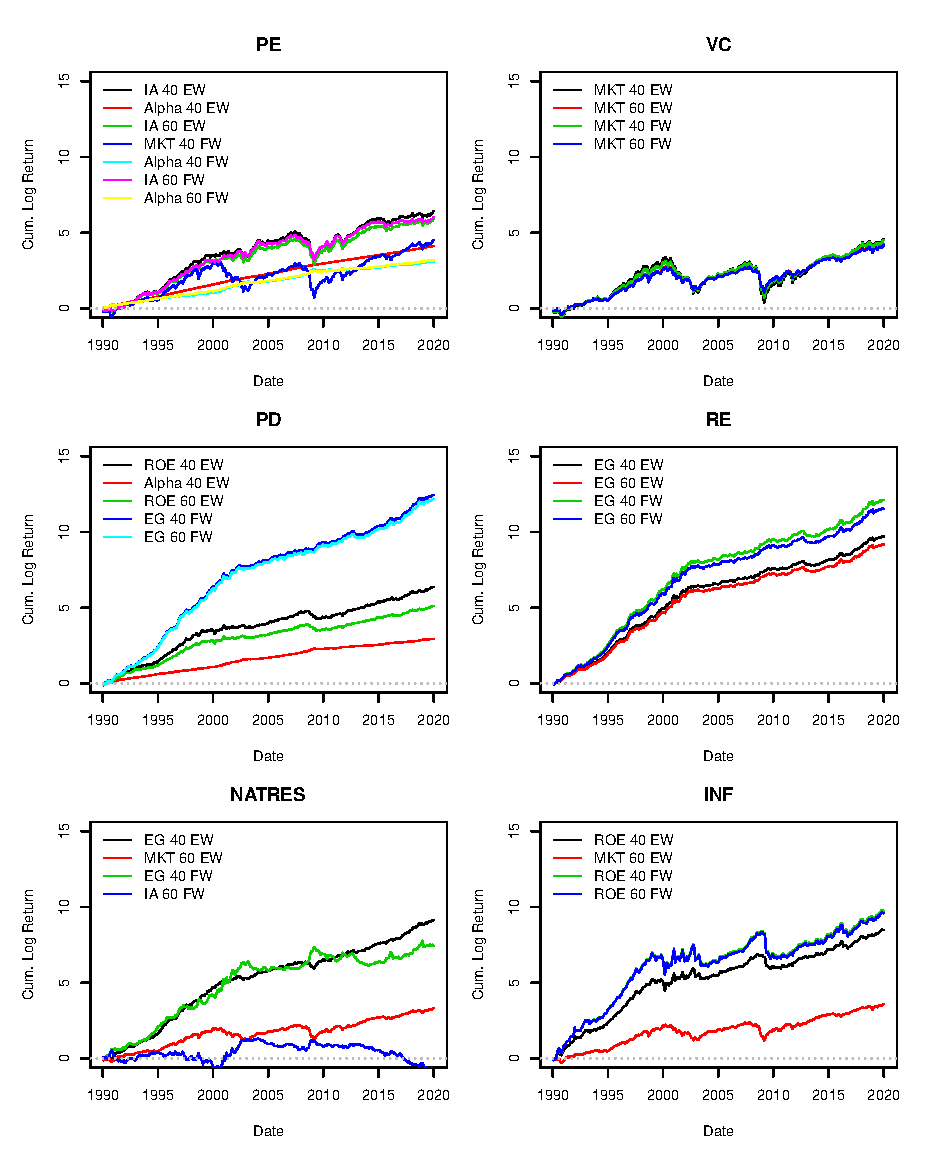
\includegraphics{eps/0_SDF_realizations_fundwise}
	\caption{Cumulative log returns for the fundwise SDF models with best out-of-sample performance as displayed in table \ref{tab:result_summary}.
	}
	\label{fig:sdf_log_returns}
\end{figure}


\begin{figure}[h]
	\centering
	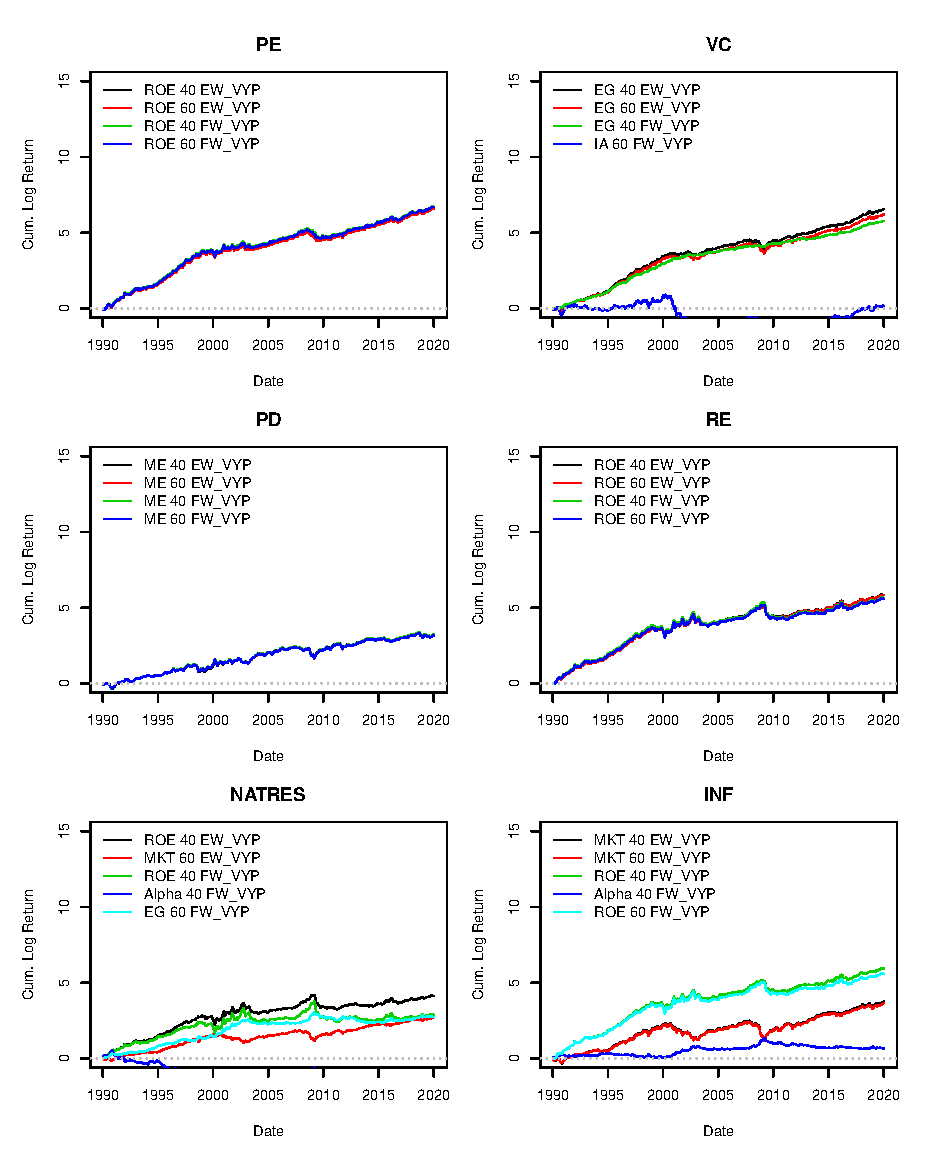
\includegraphics{eps/0_SDF_realizations_vyp}
	\caption{Cumulative log returns for the vintage year portfolio SDF models with best out-of-sample performance as displayed in table \ref{tab:result_summary_vyp}.
	}
	\label{fig:sdf_log_returns_vyp}
\end{figure}


\newpage


% latex table generated in R 3.4.2 by xtable 1.8-4 package
% Mon Apr 13 13:15:14 2020
\begin{table}[ht]
	\centering
	\begin{tabular}{lrrrlrrr}
		\hline
		Type & MKT & SE.MKT & SE.MKT.indep & Factor & Coef & SE.Coef & SE.Coef.indep \\ 
		\hline
		PE & 2.69 & 1.80 & 1.28 & MKT &  &  &  \\ 
		PE & 1.60 & 3.26 & 1.93 & ME & 1.14 & 10.32 & 1.85 \\ 
		PE & 1.98 & 2.38 & 1.11 & IA & 3.27 & 15.76 & 2.36 \\ 
		PE & 2.20 & 2.14 & 1.53 & ROE & 3.13 & 4.04 & 0.96 \\ 
		PE & 2.02 & 3.30 & 1.35 & EG & 3.48 & 7.70 & 1.82 \\ 
		PE & -0.51 & 7.02 & 0.82 & Alpha & 0.03 & 0.05 & 0.00 \\ 
		VC & 2.70 & 2.06 & 0.86 & MKT &  &  &  \\ 
		VC & 3.64 & 8.07 & 1.20 & ME & -1.36 & 10.54 & 1.31 \\ 
		VC & 2.76 & 1.97 & 0.91 & IA & -1.32 & 7.50 & 1.68 \\ 
		VC & 2.76 & 1.98 & 0.88 & ROE & -0.41 & 4.54 & 0.98 \\ 
		VC & 2.74 & 1.98 & 0.89 & EG & -0.33 & 11.41 & 2.09 \\ 
		VC & 2.79 & 6.41 & 1.14 & Alpha & -0.00 & 0.11 & 0.01 \\ 
		PD & 1.76 & 35.95 & 37.44 & MKT &  &  &  \\ 
		PD & 1.37 & 37.36 & 29.40 & ME & 0.55 & 18.77 & 27.28 \\ 
		PD & 1.67 & 15.07 & 5.13 & IA & 0.68 & 8.98 & 12.24 \\ 
		PD & 1.99 & 8.87 & 2.74 & ROE & 2.48 & 16.81 & 7.18 \\ 
		PD & 1.43 & 1.45 & 3.55 & EG & 3.83 & 16.98 & 9.35 \\ 
		PD & 0.57 & 16.29 & 4.13 & Alpha & 0.02 & 0.02 & 0.01 \\ 
		RE & 1.40 & 2.04 & 1.10 & MKT &  &  &  \\ 
		RE & 0.11 & 7.49 & 1.60 & ME & 1.55 & 6.05 & 1.58 \\ 
		RE & 1.23 & 3.32 & 2.15 & IA & 0.94 & 11.60 & 6.57 \\ 
		RE & 1.25 & 2.08 & 1.65 & ROE & 3.45 & 3.17 & 1.08 \\ 
		RE & 0.83 & 3.13 & 2.14 & EG & 4.30 & 2.71 & 4.61 \\ 
		RE & -1.59 & 3.28 & 0.53 & Alpha & 0.03 & 0.02 & 0.00 \\ 
		NATRES & -0.21 & 1.29 & 2.65 & MKT &  &  &  \\ 
		NATRES & -1.10 & 8.57 & 3.15 & ME & 1.08 & 8.95 & 5.50 \\ 
		NATRES & -0.97 & 2.92 & 2.33 & IA & 3.43 & 4.26 & 3.91 \\ 
		NATRES & -0.31 & 1.71 & 2.51 & ROE & 3.15 & 3.05 & 3.02 \\ 
		NATRES & -0.69 & 2.47 & 2.35 & EG & 4.06 & 2.94 & 2.84 \\ 
		NATRES & -2.25 & 31.58 & 12.43 & Alpha & 0.02 & 0.30 & 0.13 \\ 
		INF & 2.37 & 3.52 & 2.40 & MKT &  &  &  \\ 
		INF & 4.08 & 53.41 & 19.62 & ME & -2.54 & 55.02 & 18.69 \\ 
		INF & 1.62 & 1.00 & 2.04 & IA & 3.72 & 3.40 & 4.50 \\ 
		INF & 1.35 & 12.95 & 8.12 & ROE & 5.82 & 25.40 & 28.23 \\ 
		INF & 1.65 & 1.23 & 2.47 & EG & 5.40 & 1.64 & 5.71 \\ 
		INF & -0.79 & 64.56 & 18.25 & Alpha & 0.03 & 0.21 & 0.07 \\ 
		\hline
	\end{tabular}
	\caption{Asymptotic inference with fund-size-weighting, max quarter 40, and $D=12$.} 
	\label{tab:ai_40_fw}
\end{table}

% latex table generated in R 3.4.2 by xtable 1.8-4 package
% Mon Apr 13 13:15:14 2020
\begin{table}[ht]
	\centering
	\begin{tabular}{lrrlrrl}
		\hline
		Type & MKT & SE.MKT & Factor & Coef & SE.Coef & validation.error \\ 
		\hline
		PE & -0.09 & 0.84 & Alpha & 0.03 & 0.00 & 800 \\ 
		PE & 2.38 & 0.64 & EG & 3.28 & 0.40 & 1023 \\ 
		PE & 2.50 & 0.87 & IA & 3.30 & 1.59 & 985 \\ 
		PE & 2.21 & 0.83 & ME & 1.20 & 0.67 & 1064 \\ 
		PE & 3.07 & 0.75 & MKT & 3.07 & 0.75 & 948 \\ 
		PE & 2.30 & 0.25 & ROE & 3.11 & 0.57 & 1261 \\ 
		VC & 3.28 & 1.12 & ME & -0.88 & 1.14 & 690 \\ 
		VC & 2.70 & 0.63 & IA & -0.76 & 1.75 & 635 \\ 
		VC & 2.80 & 0.59 & MKT & 2.80 & 0.59 & 592 \\ 
		VC & 2.68 & 0.82 & EG & 0.18 & 1.91 & 653 \\ 
		VC & 2.35 & 1.93 & Alpha & 0.00 & 0.02 & 798 \\ 
		VC & 2.75 & 0.83 & ROE & 0.02 & 1.64 & 713 \\ 
		PD & 0.37 & 0.39 & Alpha & 0.02 & 0.00 & 869 \\ 
		PD & 1.38 & 0.20 & EG & 3.74 & 0.22 & 859 \\ 
		PD & 1.60 & 0.32 & IA & 1.36 & 1.95 & 1074 \\ 
		PD & 1.40 & 0.56 & ME & 0.61 & 0.92 & 1117 \\ 
		PD & 1.67 & 0.35 & MKT & 1.67 & 0.35 & 1083 \\ 
		PD & 1.75 & 0.48 & ROE & 2.54 & 0.18 & 1021 \\ 
		RE & 1.36 & 1.41 & EG & 3.77 & 2.14 & 2275 \\ 
		RE & -1.20 & 1.16 & Alpha & 0.03 & 0.01 & 2332 \\ 
		RE & 1.53 & 1.70 & IA & 2.26 & 2.17 & 2650 \\ 
		RE & 0.70 & 1.38 & ME & 1.67 & 0.69 & 2587 \\ 
		RE & 1.94 & 1.33 & MKT & 1.94 & 1.33 & 2633 \\ 
		RE & 1.51 & 0.94 & ROE & 3.46 & 1.34 & 3956 \\ 
		NATRES & -2.01 & 0.87 & Alpha & 0.02 & 0.01 & 2823 \\ 
		NATRES & -0.28 & 0.86 & EG & 3.78 & 1.13 & 2757 \\ 
		NATRES & -0.09 & 0.57 & ROE & 3.15 & 0.54 & 3020 \\ 
		NATRES & 0.20 & 0.80 & MKT & 0.20 & 0.80 & 2840 \\ 
		NATRES & -0.42 & 1.01 & IA & 3.75 & 0.60 & 2902 \\ 
		NATRES & -0.65 & 0.94 & ME & 1.04 & 0.61 & 2982 \\ 
		INF & 0.10 & 1.06 & Alpha & 0.03 & 0.01 & 2931 \\ 
		INF & 3.96 & 2.68 & ME & -1.47 & 1.61 & 3803 \\ 
		INF & 2.51 & 1.52 & IA & 4.28 & 4.52 & 4911 \\ 
		INF & 1.76 & 0.94 & ROE & 5.28 & 0.89 & 1896 \\ 
		INF & 3.37 & 2.20 & MKT & 3.37 & 2.20 & 4539 \\ 
		INF & 2.74 & 2.03 & EG & 5.13 & 1.24 & 4686 \\ 
		\hline
	\end{tabular}
	\caption{$hv$-block cross-validation with fund-size-weighting and max quarter 40.} 
	\label{tab:cv_40_fw}
\end{table}

% latex table generated in R 3.4.2 by xtable 1.8-4 package
% Mon Apr 13 13:15:14 2020
\begin{table}[ht]
	\centering
	\begin{tabular}{lrrrlrrr}
		\hline
		Type & MKT & SE.MKT & SE.MKT.indep & Factor & Coef & SE.Coef & SE.Coef.indep \\ 
		\hline
		PE & 2.51 & 1.89 & 1.48 & MKT &  &  &  \\ 
		PE & 1.47 & 5.59 & 1.82 & ME & 1.07 & 10.74 & 1.80 \\ 
		PE & 1.88 & 5.47 & 1.39 & IA & 2.81 & 18.45 & 2.45 \\ 
		PE & 2.10 & 4.48 & 1.95 & ROE & 2.34 & 7.25 & 1.47 \\ 
		PE & 1.97 & 3.85 & 1.70 & EG & 2.67 & 15.01 & 2.70 \\ 
		PE & -0.29 & 8.45 & 1.22 & Alpha & 0.03 & 0.08 & 0.01 \\ 
		VC & 2.12 & 1.43 & 0.94 & MKT &  &  &  \\ 
		VC & 3.56 & 8.69 & 1.26 & ME & -1.78 & 11.52 & 1.32 \\ 
		VC & 2.22 & 1.62 & 0.93 & IA & -2.11 & 8.48 & 1.60 \\ 
		VC & 2.42 & 1.54 & 0.81 & ROE & -1.45 & 4.83 & 0.81 \\ 
		VC & 2.44 & 1.93 & 0.89 & EG & -1.99 & 7.76 & 1.22 \\ 
		VC & 2.92 & 10.44 & 1.57 & Alpha & -0.01 & 0.03 & 0.01 \\ 
		PD & 1.67 & 14.12 & 11.35 & MKT &  &  &  \\ 
		PD & 1.27 & 10.15 & 13.21 & ME & 0.56 & 134.15 & 31.84 \\ 
		PD & 1.50 & 15.04 & 4.94 & IA & 1.31 & 9.34 & 12.21 \\ 
		PD & 1.86 & 6.79 & 2.10 & ROE & 2.19 & 8.68 & 5.84 \\ 
		PD & 1.38 & 1.44 & 3.55 & EG & 3.75 & 17.39 & 9.38 \\ 
		PD & 0.53 & 33.47 & 9.06 & Alpha & 0.02 & 0.13 & 0.03 \\ 
		RE & 1.30 & 2.58 & 1.82 & MKT &  &  &  \\ 
		RE & 0.26 & 7.13 & 1.78 & ME & 1.25 & 5.02 & 1.76 \\ 
		RE & 1.13 & 2.99 & 2.24 & IA & 0.86 & 10.15 & 6.38 \\ 
		RE & 1.13 & 2.11 & 1.95 & ROE & 2.77 & 4.38 & 1.31 \\ 
		RE & 0.74 & 3.45 & 2.27 & EG & 4.11 & 2.80 & 4.78 \\ 
		RE & -1.32 & 11.78 & 2.36 & Alpha & 0.03 & 0.03 & 0.01 \\ 
		NATRES & -0.32 & 1.75 & 2.62 & MKT &  &  &  \\ 
		NATRES & -0.85 & 22.11 & 11.30 & ME & 0.64 & 27.06 & 16.10 \\ 
		NATRES & -1.08 & 3.43 & 2.32 & IA & 3.40 & 4.46 & 3.86 \\ 
		NATRES & -0.41 & 1.91 & 2.48 & ROE & 2.72 & 3.32 & 3.16 \\ 
		NATRES & -0.73 & 2.63 & 2.40 & EG & 3.50 & 4.12 & 5.59 \\ 
		NATRES & -2.10 & 29.82 & 12.47 & Alpha & 0.02 & 0.28 & 0.13 \\ 
		INF & 2.27 & 3.12 & 2.32 & MKT &  &  &  \\ 
		INF & 3.98 & 53.63 & 19.75 & ME & -2.55 & 53.93 & 18.29 \\ 
		INF & 1.48 & 1.91 & 1.96 & IA & 4.03 & 2.43 & 4.20 \\ 
		INF & 1.29 & 21.01 & 10.81 & ROE & 5.82 & 25.08 & 24.50 \\ 
		INF & 1.61 & 1.61 & 3.02 & EG & 5.35 & 1.62 & 5.74 \\ 
		INF & -0.68 & 57.21 & 17.12 & Alpha & 0.03 & 0.03 & 0.01 \\ 
		\hline
	\end{tabular}
	\caption{Asymptotic inference with fund-size-weighting, max quarter 60, and $D=12$.} 
	\label{tab:ai_60_fw}
\end{table}

% latex table generated in R 3.4.2 by xtable 1.8-4 package
% Mon Apr 13 13:15:14 2020
\begin{table}[ht]
	\centering
	\begin{tabular}{lrrlrrl}
		\hline
		Type & MKT & SE.MKT & Factor & Coef & SE.Coef & validation.error \\ 
		\hline
		PE & -0.09 & 0.54 & Alpha & 0.03 & 0.00 & 948 \\ 
		PE & 2.07 & 0.34 & EG & 2.53 & 0.43 & 1138 \\ 
		PE & 2.10 & 0.45 & IA & 2.63 & 1.60 & 1009 \\ 
		PE & 1.83 & 0.58 & ME & 1.04 & 0.55 & 1063 \\ 
		PE & 2.64 & 0.43 & MKT & 2.64 & 0.43 & 1015 \\ 
		PE & 2.02 & 0.26 & ROE & 2.32 & 0.35 & 1560 \\ 
		VC & 2.17 & 0.44 & MKT & 2.17 & 0.44 & 654 \\ 
		VC & 2.29 & 0.61 & EG & -1.50 & 2.12 & 738 \\ 
		VC & 2.40 & 1.81 & Alpha & -0.00 & 0.02 & 931 \\ 
		VC & 3.14 & 1.01 & ME & -1.34 & 1.16 & 755 \\ 
		VC & 2.08 & 0.50 & IA & -1.75 & 2.57 & 729 \\ 
		VC & 2.33 & 0.64 & ROE & -1.00 & 1.58 & 800 \\ 
		PD & 0.32 & 0.43 & Alpha & 0.02 & 0.00 & 1093 \\ 
		PD & 1.27 & 0.31 & EG & 3.53 & 0.52 & 1084 \\ 
		PD & 1.40 & 0.40 & IA & 1.80 & 1.53 & 1159 \\ 
		PD & 1.32 & 0.71 & ME & 0.49 & 0.91 & 1256 \\ 
		PD & 1.51 & 0.51 & MKT & 1.51 & 0.51 & 1233 \\ 
		PD & 1.61 & 0.54 & ROE & 2.26 & 0.23 & 1289 \\ 
		RE & 1.17 & 1.64 & IA & 2.15 & 2.44 & 2885 \\ 
		RE & 0.63 & 1.19 & ME & 1.23 & 0.69 & 2770 \\ 
		RE & 1.04 & 1.34 & EG & 3.58 & 1.91 & 2488 \\ 
		RE & -1.12 & 1.03 & Alpha & 0.03 & 0.01 & 2949 \\ 
		RE & 1.60 & 1.27 & MKT & 1.60 & 1.27 & 2839 \\ 
		RE & 1.28 & 1.05 & ROE & 2.85 & 1.25 & 4120 \\ 
		NATRES & -1.89 & 0.68 & Alpha & 0.02 & 0.00 & 3010 \\ 
		NATRES & -0.44 & 0.68 & EG & 3.22 & 1.15 & 2880 \\ 
		NATRES & -0.68 & 0.78 & IA & 3.62 & 0.46 & 2770 \\ 
		NATRES & -0.56 & 0.72 & ME & 0.63 & 0.53 & 2882 \\ 
		NATRES & -0.29 & 0.44 & ROE & 2.72 & 0.65 & 3567 \\ 
		NATRES & -0.03 & 0.62 & MKT & -0.03 & 0.62 & 2793 \\ 
		INF & 0.21 & 1.09 & Alpha & 0.03 & 0.01 & 3694 \\ 
		INF & 1.72 & 0.95 & ROE & 5.22 & 0.95 & 2265 \\ 
		INF & 3.33 & 2.26 & MKT & 3.33 & 2.26 & 4828 \\ 
		INF & 2.73 & 2.08 & EG & 5.13 & 1.21 & 5396 \\ 
		INF & 3.86 & 2.77 & ME & -1.43 & 1.68 & 4019 \\ 
		INF & 2.35 & 1.65 & IA & 4.72 & 3.66 & 5131 \\ 
		\hline
	\end{tabular}
	\caption{$hv$-block cross-validation with fund-size-weighting and max quarter 60.} 
	\label{tab:cv_60_fw}
\end{table}



% latex table generated in R 3.4.2 by xtable 1.8-4 package
% Mon Apr 13 15:21:32 2020
\begin{table}[ht]
	\centering
	\begin{tabular}{lrrrlrrr}
		\hline
		Type & MKT & SE.MKT & SE.MKT.indep & Factor & Coef & SE.Coef & SE.Coef.indep \\ 
		\hline
		PE & 2.74 & 1.36 & 0.52 & MKT &  &  &  \\ 
		PE & 1.66 & 0.04 & 0.00 & ME & 1.42 & 0.01 & 0.00 \\ 
		PE & 2.33 & 1.09 & 0.42 & IA & 2.61 & 7.63 & 0.94 \\ 
		PE & 2.06 & 2.59 & 0.65 & ROE & 2.19 & 4.07 & 0.61 \\ 
		PE & 2.15 & 2.08 & 0.54 & EG & 2.70 & 6.66 & 1.10 \\ 
		PE & -0.01 & 27.12 & 1.47 & Alpha & 0.03 & 0.09 & 0.01 \\ 
		VC & 3.08 & 1.51 & 0.49 & MKT &  &  &  \\ 
		VC & 3.50 & 4.31 & 0.69 & ME & -1.65 & 6.31 & 0.72 \\ 
		VC & 2.91 & 1.38 & 0.56 & IA & -1.92 & 4.40 & 1.34 \\ 
		VC & 3.23 & 1.74 & 0.52 & ROE & -1.29 & 3.49 & 0.79 \\ 
		VC & 3.08 & 1.47 & 0.49 & EG & 0.18 & 7.47 & 1.65 \\ 
		VC & 3.49 & 5.50 & 0.55 & Alpha & -0.01 & 0.03 & 0.00 \\ 
		PD & 1.55 & 6.22 & 2.66 & MKT &  &  &  \\ 
		PD & 0.50 & 22.42 & 4.84 & ME & 1.62 & 12.69 & 4.67 \\ 
		PD & 1.13 & 8.42 & 2.05 & IA & 3.43 & 11.35 & 4.30 \\ 
		PD & 1.21 & 4.93 & 2.39 & ROE & 1.98 & 7.79 & 2.76 \\ 
		PD & 1.17 & 13.58 & 5.44 & EG & 3.16 & 10.23 & 10.14 \\ 
		PD & -0.26 & 1.72 & 0.25 & Alpha & 0.02 & 0.01 & 0.00 \\ 
		RE & 1.13 & 3.64 & 1.28 & MKT &  &  &  \\ 
		RE & 0.17 & 7.75 & 1.38 & ME & 1.20 & 4.19 & 1.37 \\ 
		RE & 0.92 & 2.74 & 1.13 & IA & 1.24 & 10.30 & 3.07 \\ 
		RE & 0.71 & 4.01 & 1.43 & ROE & 2.68 & 3.81 & 0.97 \\ 
		RE & 0.67 & 5.16 & 1.45 & EG & 3.27 & 3.75 & 2.83 \\ 
		RE & -1.30 & 7.86 & 0.84 & Alpha & 0.03 & 0.03 & 0.00 \\ 
		NATRES & 1.92 & 2.40 & 1.47 & MKT &  &  &  \\ 
		NATRES & 1.01 & 8.90 & 11.40 & ME & 1.37 & 12.18 & 16.33 \\ 
		NATRES & 1.61 & 18.93 & 13.81 & IA & 2.07 & 163.96 & 115.42 \\ 
		NATRES & 1.59 & 1.43 & 1.76 & ROE & 1.92 & 4.67 & 3.46 \\ 
		NATRES & 1.48 & 11.76 & 9.51 & EG & 2.27 & 85.24 & 71.19 \\ 
		NATRES & -0.05 & 6.80 & 2.94 & Alpha & 0.02 & 0.08 & 0.04 \\ 
		INF & 1.69 & 1.74 & 4.30 & MKT &  &  &  \\ 
		INF & 0.90 & 8.81 & 4.23 & ME & 1.05 & 7.87 & 5.74 \\ 
		INF & 1.71 & 3.83 & 6.06 & IA & -0.12 & 14.76 & 11.99 \\ 
		INF & 1.20 & 9.61 & 4.51 & ROE & 3.92 & 27.10 & 15.10 \\ 
		INF & 1.18 & 9.84 & 5.94 & EG & 3.35 & 11.00 & 17.20 \\ 
		INF & -0.77 & 18.40 & 4.34 & Alpha & 0.03 & 0.01 & 0.00 \\ 
		\hline
	\end{tabular}
	\caption{Asymptotic inference with equal-weighting, max quarter 40, and $D=12$.} 
	\label{tab:ai_40_ew}
\end{table}

% latex table generated in R 3.4.2 by xtable 1.8-4 package
% Mon Apr 13 15:21:32 2020
\begin{table}[ht]
	\centering
	\begin{tabular}{lrrlrrl}
		\hline
		Type & MKT & SE.MKT & Factor & Coef & SE.Coef & validation.error \\ 
		\hline
		PE & -0.02 & 0.57 & Alpha & 0.03 & 0.00 & 980 \\ 
		PE & 2.13 & 0.17 & EG & 2.73 & 0.20 & 1050 \\ 
		PE & 2.40 & 0.22 & IA & 2.69 & 0.40 & 1039 \\ 
		PE & 1.75 & 0.33 & ME & 1.50 & 0.24 & 1074 \\ 
		PE & 2.77 & 0.17 & MKT & 2.77 & 0.17 & 1137 \\ 
		PE & 2.00 & 0.26 & ROE & 2.27 & 0.45 & 1313 \\ 
		VC & 3.35 & 0.83 & ME & -1.30 & 1.21 & 1215 \\ 
		VC & 2.84 & 0.39 & IA & -1.51 & 1.43 & 1006 \\ 
		VC & 2.99 & 0.48 & MKT & 2.99 & 0.48 & 946 \\ 
		VC & 2.80 & 0.74 & EG & 0.72 & 1.75 & 1034 \\ 
		VC & 2.84 & 1.67 & Alpha & -0.00 & 0.02 & 1293 \\ 
		VC & 3.01 & 0.72 & ROE & -0.67 & 1.70 & 1161 \\ 
		PD & -0.28 & 0.23 & Alpha & 0.02 & 0.00 & 2850 \\ 
		PD & 1.08 & 0.40 & EG & 3.16 & 0.41 & 2956 \\ 
		PD & 1.11 & 0.30 & IA & 3.35 & 0.61 & 2954 \\ 
		PD & 0.52 & 0.25 & ME & 1.63 & 0.14 & 3040 \\ 
		PD & 1.43 & 0.46 & MKT & 1.43 & 0.46 & 3209 \\ 
		PD & 1.10 & 0.54 & ROE & 2.05 & 0.36 & 2893 \\ 
		RE & 0.85 & 0.64 & EG & 3.06 & 0.37 & 1078 \\ 
		RE & -1.09 & 0.71 & Alpha & 0.03 & 0.01 & 1725 \\ 
		RE & 1.15 & 0.85 & IA & 1.65 & 0.60 & 1820 \\ 
		RE & 0.42 & 0.58 & ME & 1.37 & 0.69 & 1779 \\ 
		RE & 1.34 & 0.76 & MKT & 1.34 & 0.76 & 1919 \\ 
		RE & 0.72 & 0.41 & ROE & 2.87 & 1.03 & 1902 \\ 
		NATRES & 0.07 & 0.65 & Alpha & 0.02 & 0.00 & 8024 \\ 
		NATRES & 1.63 & 0.47 & EG & 2.24 & 0.41 & 7108 \\ 
		NATRES & 1.62 & 0.59 & ROE & 2.26 & 1.42 & 8287 \\ 
		NATRES & 2.05 & 0.46 & MKT & 2.05 & 0.46 & 7672 \\ 
		NATRES & 1.81 & 0.51 & IA & 1.93 & 0.86 & 7824 \\ 
		NATRES & 1.21 & 0.76 & ME & 1.44 & 0.60 & 9138 \\ 
		INF & -0.23 & 1.08 & Alpha & 0.03 & 0.01 & 4554 \\ 
		INF & 1.61 & 1.42 & ME & 0.89 & 0.76 & 3526 \\ 
		INF & 2.26 & 0.95 & IA & -0.60 & 1.26 & 3428 \\ 
		INF & 1.56 & 0.97 & ROE & 3.81 & 2.19 & 3364 \\ 
		INF & 2.21 & 1.01 & MKT & 2.21 & 1.01 & 3395 \\ 
		INF & 1.73 & 1.08 & EG & 3.22 & 0.71 & 4197 \\ 
		\hline
	\end{tabular}
	\caption{$hv$-block cross-validation with equal-weighting and max quarter 40.} 
	\label{tab:cv_40_ew}
\end{table}

% latex table generated in R 3.4.2 by xtable 1.8-4 package
% Mon Apr 13 15:21:32 2020
\begin{table}[ht]
	\centering
	\begin{tabular}{lrrrlrrr}
		\hline
		Type & MKT & SE.MKT & SE.MKT.indep & Factor & Coef & SE.Coef & SE.Coef.indep \\ 
		\hline
		PE & 2.35 & 2.48 & 0.64 & MKT &  &  &  \\ 
		PE & 1.59 & 3.45 & 0.62 & ME & 1.03 & 7.03 & 0.65 \\ 
		PE & 2.03 & 3.80 & 0.57 & IA & 2.28 & 9.28 & 1.07 \\ 
		PE & 1.83 & 5.48 & 0.87 & ROE & 1.61 & 6.39 & 0.88 \\ 
		PE & 1.89 & 5.16 & 0.66 & EG & 2.19 & 8.27 & 1.18 \\ 
		PE & 0.24 & 14.32 & 0.91 & Alpha & 0.02 & 0.05 & 0.01 \\ 
		VC & 2.20 & 0.97 & 0.58 & MKT &  &  &  \\ 
		VC & 3.24 & 4.77 & 0.68 & ME & -2.42 & 6.69 & 0.64 \\ 
		VC & 1.93 & 1.24 & 0.56 & IA & -3.50 & 5.25 & 1.11 \\ 
		VC & 2.67 & 1.31 & 0.47 & ROE & -2.50 & 3.38 & 0.80 \\ 
		VC & 2.40 & 0.93 & 0.53 & EG & -2.42 & 5.26 & 0.98 \\ 
		VC & 3.48 & 2.02 & 0.18 & Alpha & -0.02 & 0.01 & 0.00 \\ 
		PD & 1.18 & 53.03 & 13.01 & MKT &  &  &  \\ 
		PD & 0.30 & 48.26 & 12.32 & ME & 1.35 & 17.73 & 13.57 \\ 
		PD & 0.80 & 45.54 & 8.13 & IA & 3.27 & 37.72 & 7.72 \\ 
		PD & 0.89 & 13.97 & 2.80 & ROE & 1.53 & 15.14 & 3.06 \\ 
		PD & 0.85 & 72.30 & 15.48 & EG & 2.52 & 12.41 & 10.47 \\ 
		PD & -0.37 & 0.44 & 0.39 & Alpha & 0.02 & 0.02 & 0.00 \\ 
		RE & 1.00 & 4.00 & 1.33 & MKT &  &  &  \\ 
		RE & 0.20 & 8.59 & 1.70 & ME & 0.99 & 4.59 & 1.89 \\ 
		RE & 0.81 & 3.45 & 1.28 & IA & 1.10 & 10.34 & 3.06 \\ 
		RE & 0.58 & 5.57 & 1.81 & ROE & 2.33 & 7.17 & 1.74 \\ 
		RE & 0.56 & 6.32 & 1.45 & EG & 3.14 & 5.26 & 3.12 \\ 
		RE & -1.12 & 0.85 & 0.11 & Alpha & 0.02 & 0.00 & 0.00 \\ 
		NATRES & 1.37 & 1.48 & 1.52 & MKT &  &  &  \\ 
		NATRES & 0.96 & 6.20 & 4.07 & ME & 0.65 & 9.75 & 5.99 \\ 
		NATRES & 1.10 & 15.72 & 11.67 & IA & 2.11 & 149.64 & 105.24 \\ 
		NATRES & 1.19 & 1.56 & 1.63 & ROE & 1.20 & 8.96 & 5.16 \\ 
		NATRES & 1.14 & 2.72 & 2.12 & EG & 1.48 & 26.71 & 18.94 \\ 
		NATRES & 0.33 & 0.09 & 0.10 & Alpha & 0.01 & 0.00 & 0.00 \\ 
		INF & 1.58 & 1.74 & 4.26 & MKT &  &  &  \\ 
		INF & 0.82 & 9.28 & 4.18 & ME & 1.02 & 7.98 & 5.72 \\ 
		INF & 1.58 & 3.19 & 5.87 & IA & 0.03 & 12.14 & 11.65 \\ 
		INF & 1.16 & 9.56 & 4.52 & ROE & 3.77 & 30.53 & 14.73 \\ 
		INF & 1.14 & 9.91 & 6.11 & EG & 3.19 & 12.07 & 18.98 \\ 
		INF & -0.45 & 31.81 & 9.95 & Alpha & 0.02 & 0.21 & 0.09 \\ 
		\hline
	\end{tabular}
	\caption{Asymptotic inference with equal-weighting, max quarter 60, and $D=12$.} 
	\label{tab:ai_60_ew}
\end{table}

% latex table generated in R 3.4.2 by xtable 1.8-4 package
% Mon Apr 13 15:21:32 2020
\begin{table}[ht]
	\centering
	\begin{tabular}{lrrlrrl}
		\hline
		Type & MKT & SE.MKT & Factor & Coef & SE.Coef & validation.error \\ 
		\hline
		PE & 0.18 & 0.47 & Alpha & 0.02 & 0.00 & 1310 \\ 
		PE & 1.84 & 0.27 & EG & 2.22 & 0.18 & 1228 \\ 
		PE & 2.02 & 0.22 & IA & 2.33 & 0.39 & 1226 \\ 
		PE & 1.57 & 0.28 & ME & 1.08 & 0.26 & 1324 \\ 
		PE & 2.30 & 0.29 & MKT & 2.30 & 0.29 & 1275 \\ 
		PE & 1.74 & 0.32 & ROE & 1.66 & 0.31 & 1441 \\ 
		VC & 2.13 & 0.66 & MKT & 2.13 & 0.66 & 1070 \\ 
		VC & 2.14 & 0.76 & EG & -1.67 & 2.02 & 1223 \\ 
		VC & 2.85 & 1.63 & Alpha & -0.01 & 0.02 & 1517 \\ 
		VC & 2.95 & 0.78 & ME & -2.02 & 1.22 & 1247 \\ 
		VC & 1.84 & 0.59 & IA & -2.63 & 2.64 & 1189 \\ 
		VC & 2.48 & 0.71 & ROE & -1.88 & 1.54 & 1302 \\ 
		PD & -0.45 & 0.35 & Alpha & 0.02 & 0.00 & 3550 \\ 
		PD & 0.72 & 0.58 & EG & 2.48 & 0.40 & 3674 \\ 
		PD & 0.68 & 0.52 & IA & 3.08 & 0.44 & 3595 \\ 
		PD & 0.19 & 0.39 & ME & 1.32 & 0.24 & 3719 \\ 
		PD & 1.00 & 0.66 & MKT & 1.00 & 0.66 & 3578 \\ 
		PD & 0.75 & 0.65 & ROE & 1.57 & 0.30 & 3483 \\ 
		RE & 0.95 & 0.81 & IA & 1.43 & 0.59 & 1992 \\ 
		RE & 0.39 & 0.50 & ME & 1.10 & 0.58 & 1996 \\ 
		RE & 0.69 & 0.62 & EG & 2.93 & 0.40 & 1104 \\ 
		RE & -0.99 & 0.68 & Alpha & 0.02 & 0.01 & 2097 \\ 
		RE & 1.14 & 0.74 & MKT & 1.14 & 0.74 & 2080 \\ 
		RE & 0.57 & 0.42 & ROE & 2.55 & 0.96 & 2026 \\ 
		NATRES & 0.35 & 0.71 & Alpha & 0.01 & 0.00 & 9920 \\ 
		NATRES & 1.24 & 0.44 & EG & 1.45 & 0.43 & 9102 \\ 
		NATRES & 1.23 & 0.50 & IA & 1.97 & 0.85 & 9111 \\ 
		NATRES & 0.97 & 0.84 & ME & 0.76 & 0.65 & 11459 \\ 
		NATRES & 1.17 & 0.48 & ROE & 1.55 & 1.40 & 10806 \\ 
		NATRES & 1.44 & 0.39 & MKT & 1.44 & 0.39 & 8861 \\ 
		INF & 0.02 & 1.24 & Alpha & 0.03 & 0.01 & 5912 \\ 
		INF & 1.56 & 1.00 & ROE & 3.50 & 2.58 & 4003 \\ 
		INF & 2.14 & 1.08 & MKT & 2.14 & 1.08 & 3510 \\ 
		INF & 1.77 & 1.21 & EG & 2.97 & 0.97 & 4920 \\ 
		INF & 1.56 & 1.48 & ME & 0.85 & 0.81 & 3660 \\ 
		INF & 2.13 & 1.07 & IA & -0.31 & 1.19 & 3532 \\ 
		\hline
	\end{tabular}
	\caption{$hv$-block cross-validation with equal-weighting and max quarter 60.} 
	\label{tab:cv_60_ew}
\end{table}


\end{document}
